\documentclass[a4paper, 10pt, notitlepage]{article}

\usepackage{moreverb} %para importar codigo

\usepackage{pepotina} %paquete personal para la caratula del DC

\usepackage[spanish,activeacute]{babel}
\usepackage{babel} %paquete de idioma

\usepackage[latin1]{inputenc}

\usepackage[normalem]{ulem}
\usepackage{ulem}

%\usepackage{color}

\usepackage{hyperref}
%\usepackage[all]{hypcap}

\usepackage{caeycaeBD}

\usepackage{fancyhdr} %linea sup con comentarios

\usepackage{lscape} %para hoja apaisada

\usepackage{framed} %para crear cajas de texto

\usepackage{lastpage} %ultima pagina

%\usepackage{pstricks}
%\usepackage{uml} %UML

\usepackage{listings}
%\lstset{
%  breaklines=true,                                     % line wrapping on
%  language=ocl,
%  frame=ltrb,
%  framesep=5pt,
%  basicstyle=\normalsize,
%  keywordstyle=\ttfamily\color{OliveGreen},
%  identifierstyle=\ttfamily\color{CadetBlue}\bfseries,
%  commentstyle=\color{Brown},
%  stringstyle=\ttfamily,
%  showstringspaces=ture
%}

\addtolength{\topmargin}{-50pt} 
\addtolength{\textwidth}{145pt}
\addtolength{\textheight}{120pt}
\addtolength{\oddsidemargin}{-70pt}

%\newcommand{\minix}{\textsl{minix }}

%%% Encabezado y pie de p'agina
\pagestyle{fancy}
\fancyhead[LO]{Base de Datos}
\fancyhead[C]{}
\fancyhead[RO]{P\'agina \thepage\ de \pageref{LastPage}}
\renewcommand{\headrulewidth}{0.4pt}
\fancyfoot{}

\newcommand{\FALTA}{{\bf FALTA FALTA FALTA FALTA FALTA FALTA FALTA FALTA }}
\def\var#1{\textsl{#1}}


\begin{document}

\universidad{Universidad de Buenos Aires}
\facultad{Facultad de ciencias exactas y naturales}
\departamento{Departamento de Computacion}
\materia{Base de Datos}
\resumen{El presente trabajo pr�ctico consiste en el desarrollo de una base de datos desarrollada en SQL para una empresa de transporte. Lo primero que se hizo fue un diagrama entidad relaci�n de los requerimientos. Luego a partir de �ste �ltimo se construy� el modelo relacional. Finalmente se llev� lo anterior a un dise�o f�sico utilizando el motor de base de datos SQL server 2005.}
\keys{MER, DER, MR, SQL, Base de Datos, Base de Datos Relacional}
\titulo{Tp1}
\subtitulo{Tp 1: Empresa de Transportes}
\grupo{Numero de grupo: 1}
\fecha{2do Cuatrimeste 2011}
\footspace{1cm}
\integrante{Piotrkowski, Kevin}{204/06}{marcoskevin@gmail.com}
\integrante{Rugnone, Mart�n}{665/04}{mrugnone@hotmail.com}
\integrante{Alvarez, Mar�a de los Angeles}{264/05}{mdelosaalvarez@hotmail.com}
\integrante{Engler, Christian}{314/05}{caeycae@gmail.com}

\maketitle{}

\tableofcontents

\newpage


\section{Introducci�n}

\begin{quotation}
\textit{``El Buffer Manager es uno de los componentes m�s importantes dentro de un motor de BD. Su principal funci�n es administrar un espacio de memoria de la BD, utilizado como una especie de memoria cach�. El objetivo es que las diferentes aplicaciones que usan la BD y requieren p�ginas de disco, puedan recuperar la p�gina de este espacio de memoria y accedan lo menos posible al disco.''}
\end{quotation}

En este informe analizaremos el tipo de trazas definidas por distintos algoritmos(NBLJ, File Scan, Index Scan, etc) y las diferencias de permonance(medida seg�n el hit-rate) que se obtienen al probar las estrategias de reemplazo MRU, LRU y FIFO. Los resultados obtenidos por las diferentes estrategias de reemplazo nos permitir�n sacar conclusiones y definir heur�sticas sobre la mejor estrategia a usar para cada algoritmo.

En la realizaci�n de este trabajo pr�ctico empezamos por realizar la implementaci�n de las estrategias LRU y MRU con sus respectivos casos de test, desarrollamos un parser de trazas almacenadas en archivos de texto plano, definimos trazas representativas de los algorimos a evaluar, luego analizamos las trazas definidas con las 3 estrategias de reemplazo mencionadas anteriormente, para finalmente expresar las conclusiones obtenidas durante la realizaci�n del trabajo pr�ctico.

\section{Hip�tesis}
Consideramos los RELEASE de los bloques como una referencia al mismo por lo cu�l inciden en las distintas estrategias de reemplazo.
Ejemplo de traza:
REQUEST [R,1]
REQUEST [R,2]
RELEASE [R,2]
RELEASE [R,1]

Si se utilizara una estrategia de reemplazo MRU, el primero en ser desalojado ser�a el bloque 1 de R. 
En cambio, si la estrategia de reemplazo es LRU, el bloque que se desaloja es el 2.





\section{Hip�tesis}
\begin{enumerate}
	\item Una ruta es un camino posible para ir desde un punto a otro.
	\item Un recorrido no puede comenzar y finalizar en el mismo lugar.
	\item Con lo que respecta a las condiciones del a�o seg�n el periodo, este �ltimo se tom� como las estaciones del a�o. Es decir: invierno, oto�o, primavera y verano.
	\item No nos interesa discriminar el nombre del apellido de un chofer, pues no se cuenta con ning�n requerimiento para realizar dicha separaci�n(ej: alguna consulta para filtrar viajes por apellido del chofer).		
	\item Consideramos que \textbf{estado} del veh�culo se refiere a una descripci�n general del mismo(ej:buen estado, averiado, abollado,...) en vez de referirse al discriminante que separa a los veh�culos en: ``en uso'' y ``en reparaci�n''.
\end{enumerate}


\newpage

\section{MER}

\subsection{Decisiones de Dise�o}

\begin{enumerate}
	\item Ruta es d�bil en relaci�n a un recorrido porque s�lo sirve como una forma de ir desde el origen del recorrido a su destino.
	\item Contingencia es una entidad d�bil porque puede haber una cantidad arbitraria de ellas por cada viaje realizado(en contraposici�n a una lista de contingencias predefinidas ej:choque, bloqueo de ruta, control policial, etc) y las mismas no tienen sentido sin su viaje relacionado.
	\item La ruta tiene asociado un clima por cada periodo del a�o. Como se menciono en las hipotesis el periodo son las estaciones del a�o.\\ Para ello contamos con tres entidades: ruta, clima y estaci�n. Estas tres siempres est�n vinculadas juntas. Es decir, para cada (ruta,clima) existe una instancia de estaci�n, por cada (clima, estaci�n) se vincula a una ruta y por cada par (ruta, estacion) hay un clima asociado. Por tal motivo es que decidimos modelarlo como una ternaria.
	\item Con lo que respecta al chofer y la licencia, nos pareci� m�s acorde separarlas en dos entidad pese a que en los requerimientos no queda clara dicha separaci�n. Lo realizamos as� para mayor claridad.
	\item Con respecto al dise�o de la entidad \textbf{Direcci�n} primero se opt� por hacerla d�bil de la ciudad.			
	
\begin{center}
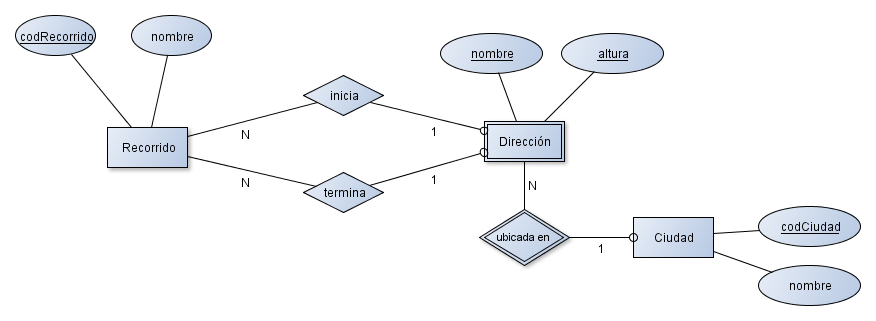
\includegraphics[scale=0.50]{img/RecorridoDirDebil.png}
\end{center}

Al poner como clave primaria de \textbf{Direccion} su altura y nombre junto a la clave primaria de la ciudad, propag�bamos estas tres claves como for�neas en otras entidad vinculadas.

Luego optamos por dejar \textbf{Direcci�n} como una entidad fuerte con una clave primaria \textbf{codDir} para as� evitar la propagaci�n de claves y obtener un dise�o m�s sencillo.

\begin{center}
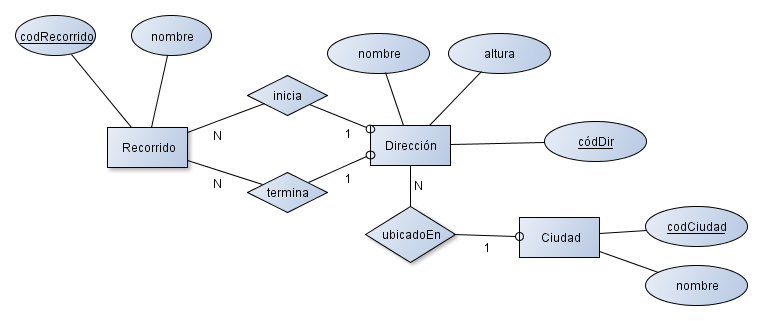
\includegraphics[scale=0.50]{img/RecorridoDirFuerte.png}
\end{center}

Vale aclarar que este dise�o admite tuplas duplicados con el mismo codDir, altura, nombre y c�digo de ciudad, sin embargo podemos impedir dicha situaci�n agregando una restricci�n adicional al DER.
  
\item Decidimos no guardar la historia de las reparaciones. Hubieramos podido hacerla de esta manera.

\begin{center}
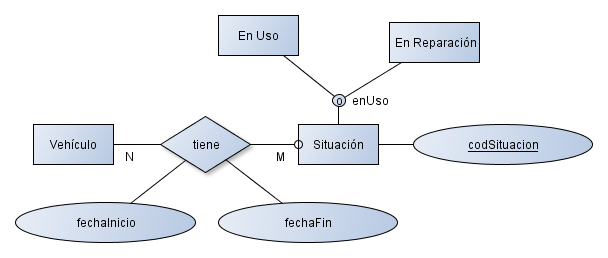
\includegraphics[scale=0.50]{img/ReparacionConHistoria.png}
\end{center}

En este dise�o hubieramos necesitado agregar restricciones para asegurar que para toda fecha posterior a $Vehiculo.fechaAlta$ el $Vehiculo$ debe tener \textbf{solo y exactamente una} $Situacion$

Pero como no hay requerimientos expl�citos por los cuales necesitemos guardar la historia, decidimos simplificar el dise�o de la siguiente manera:

\begin{center}
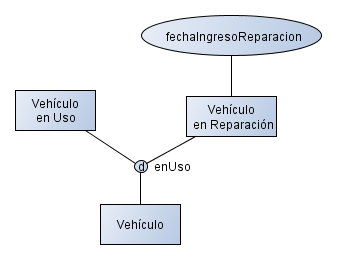
\includegraphics[scale=0.50]{img/ReparacionSinHistoria.png}
\end{center}

\item Consideramos originalmente particionar los viajes en planificados y realizados, como se muestra en el siguiente diagrama:

\begin{center}
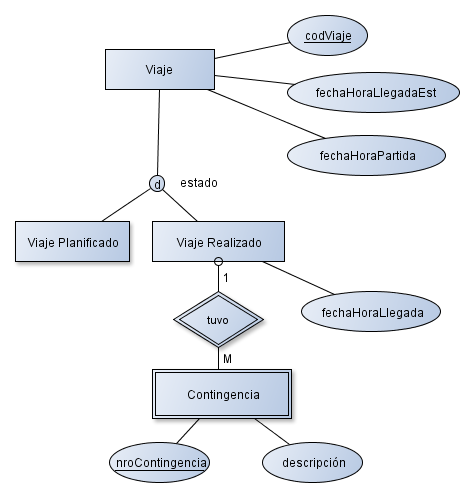
\includegraphics[scale=0.50]{img/viajePlanificado-Realizado.png}
\end{center}

Nos pareci� mejor considerar los viajes realizados como una especializaci�n de los planificados(todos los viajes son planificados y algunos de ellos adem�s pueden ser realizados). Esto lo dise�amos como una relaci�n de overlapping con una sola entidad llamada \textbf{Viaje Realizado}, describiendo que todos los viajes realizados heredan los mismos atributos que un viaje planificado, pero solo algunos viajes planificados tienen su correspondiente realizado.

\begin{center}
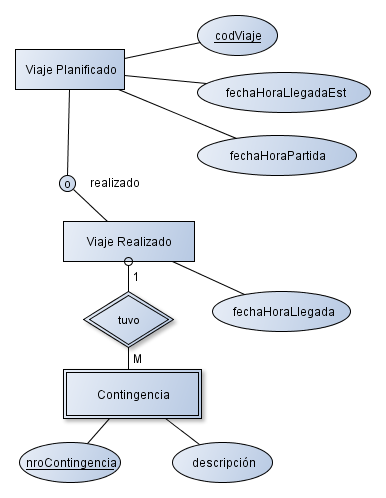
\includegraphics[scale=0.55]{img/viaje-Planificado-Realizado.png}
\end{center}

\item $(Chofer/Viaje Planificado)/Control$ es una agregaci�n pues no toda relacion $Chofer/Viaje Planificado$ tiene controles asociados.
Adem�s $Control$ es una Entidad asociada a la interrelacion entra $Vaje Planificado$ y $Control$ y no a una de ellas en particular.

\end{enumerate}

\subsection{DER}

\begin{center}
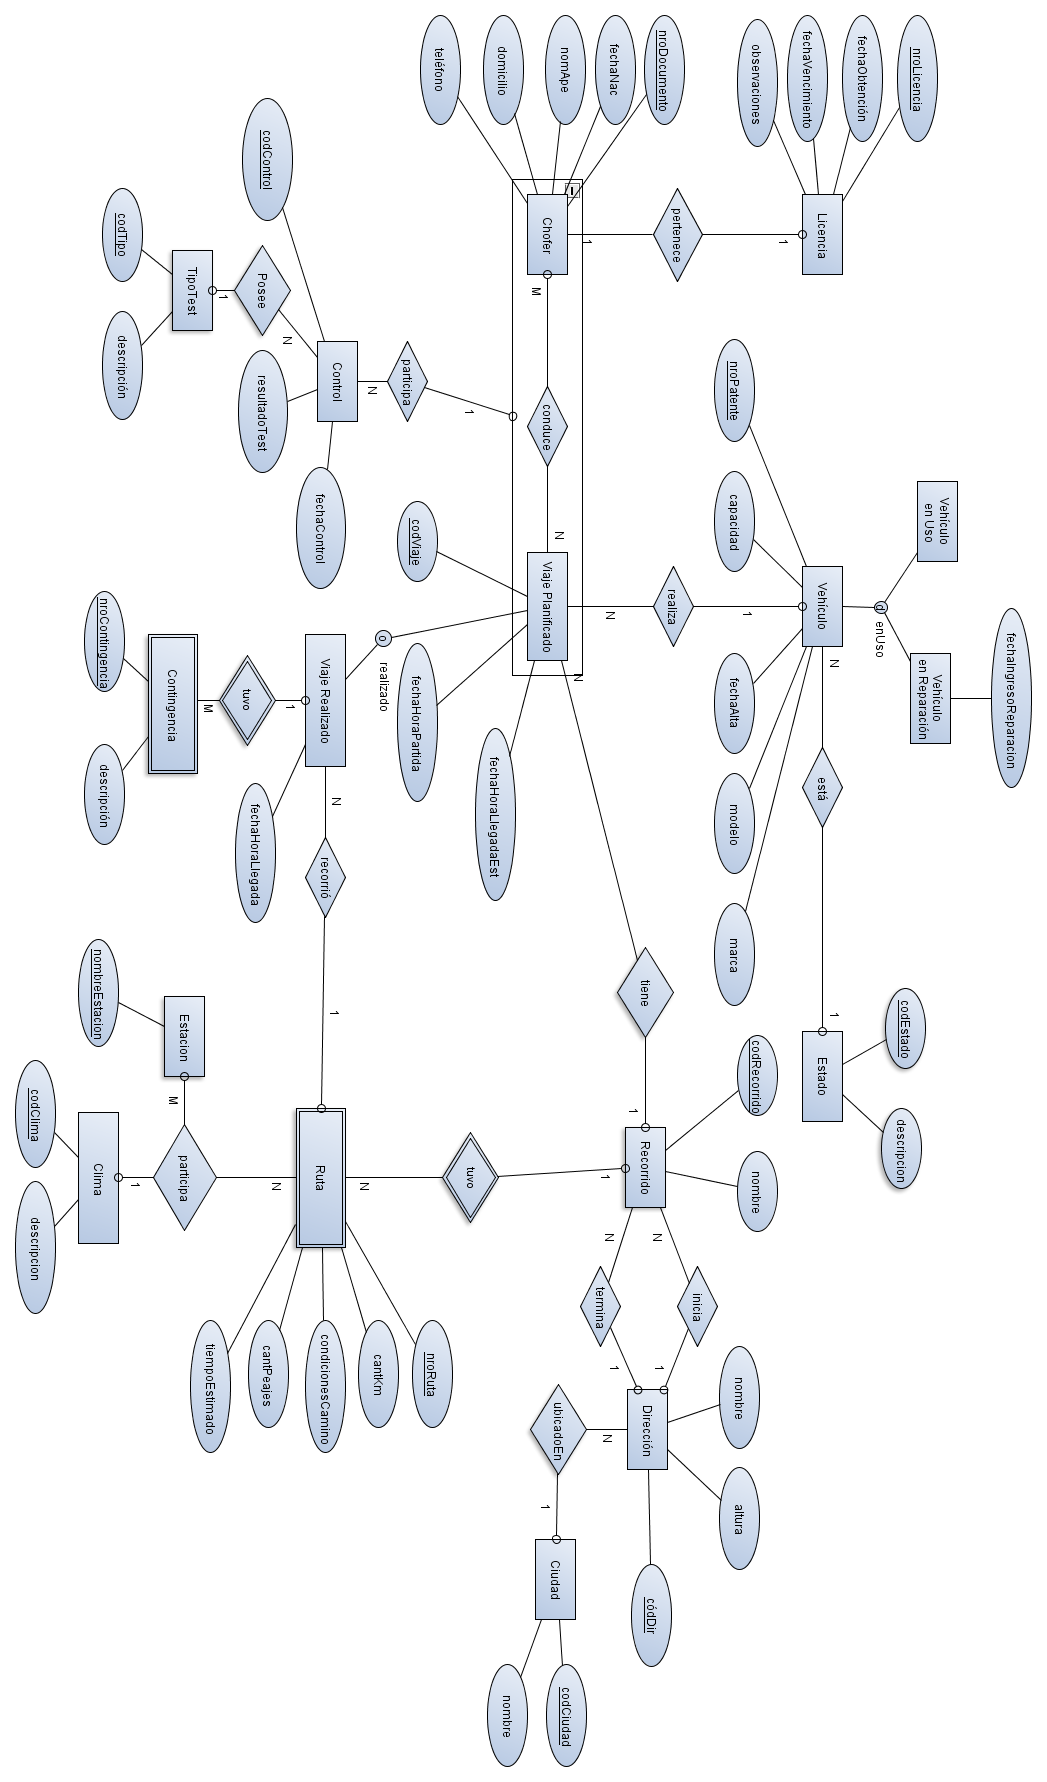
\includegraphics[height=0.95\textheight]{img/der.png}
\end{center}

\subsection{Restricciones}

\begin{enumerate}
	\item Dado 2 recorridos con distinto codigo, su origen y destino no pueden ser los mismos. Es decir, no puede haber dos recorridos ``iguales''con distinto c�digo.
	\item Para todo recorrido, el origen no puede ser igual al destino
	\item El recorrido de la ruta de todo viaje realizado debe ser igual al recorrido del viaje planificado.
	\item Para todo recorrido que tiene un viaje planificado asociado, existe una ruta.
	\item Para todo viaje la cantidad de conductores debe ser entre 1 y 3 y la fechaHoraLlegadaEst debe ser mayor a fechaHoraPartida.
	\item Para todo viaje realizado la fechaHoraLlegada debe ser mayor a fechaHoraPartida.
	\item Para todo viaje planificado que no esta realizado el vehiculo utilizado debe estar en uso.	
	\item Para todo vehiculo en reparacion la fecha de ingreso es mayor a la fecha de alta.
	\item Para toda licencia, la fecha de obtencion es menor a la fecha de vencimiento
	\item Para todo chofer, la fecha de nacimiento es menor que la fecha de obtenci�n de su licencia
	\item Para toda ruta, hay un �nico clima para todo per�odo definido
	\item Para todo control, su fecha de realizaci�n debe ser anterior a la fecha de partida del viaje que se est� controlando  
	\item La entidad Esaci�n puede tomar los valores, \textit{verano}, \textit{invierno}, \textit{oto�o} y \textit{primavera}
\end{enumerate}


\newpage

\section{MR}

\subsection{Esquema Relaci�n}

\begin{mr}{Agencia de Viajes}

\entidad{Licencia}{\pk{nroLicencia}, fechaObtencion, fechaVencimiento, observaciones}
\entidadPK{nroLicencia}
\entidadCK{nroLicencia}

\entidad{Chofer}{\pk{nroDocumento}, fechaNac, nomApe, domicilio, telefono, \fk{nroLicencia}}
\entidadPK{nroDocumento}
\entidadCK{nroDocumento}
\entidadFK{nroLicencia}

\entidad{Conduce}{\pfk{nroDocumento}, \pfk{codViaje}}
\entidadPK{(nroDocumento, codViaje)}
\entidadCK{(nroDocumento, codViaje)}
\entidadFK{nroDocumento, codViaje}

\entidad{Control}{\pk{codControl}, \fk{nroDocumento}, \fk{codViaje}, \fk{codTipo}, resultadoTest, fechaControl}
\entidadPK{codControl}
\entidadCK{codControl}
\entidadFK{(nroDocumento, codViaje), codTipo}

\entidad{TipoTest}{\pk{codTipo}, descripcion}
\entidadPK{codTipo}
\entidadCK{codTipo}

\entidad{Contingencia}{\pk{nroContingencia}, \pfk{codViaje}, descripcion}
\entidadPK{(nroContingencia, codViaje)}
\entidadCK{(nroContingencia, codViaje)}
\entidadFK{codViaje}

\entidad{Direccion}{\pk{codDir}, nombre, altura, \fk{codCiudad}}
\entidadPK{codDir}
\entidadCK{codDir}
\entidadFK{codCiudad}

\entidad{Ciudad}{\pk{codCiudad}, nombre}
\entidadPK{codCiudad}
\entidadCK{codCiudad}

\entidad{Recorrido}{\pk{codRecorrido}, nombre, \fk{codDirOrigien}, \fk{codDirDestino}}
\entidadPK{codRecorrido}
\entidadCK{codRecorrido}
\entidadFK{codDirOrigien, codDirDestino}

\entidad{Ruta}{\pk{nroRuta}, \pfk{codRecorrido}, cantKm, condicionesCamino, cantPeajes, tiempoEstimado}
\entidadPK{(nroRuta, codRecorrido)}
\entidadCK{(nroRuta, codRecorrido)}
\entidadFK{codRecorrido}

\entidad{Estado}{\pk{codEstado}, descripcion}
\entidadPK{codEstado}
\entidadCK{codEstado}

\entidad{Vehiculo}{\pk{nroPatente}, modelo, marca, capacidad, fechaAlta, \fk{codEstado}, enUso}
\entidadPK{nroPatente}
\entidadCK{nroPatente}
\entidadFK{codEstado}

\entidad{VehiculoEnReparacion}{\pfk{nroPatente}, fechaIngresoReparacion}
\entidadPK{nroPatente}
\entidadCK{nroPatente}
\entidadFK{nroPatente}

\entidad{ViajePlanificado}{\pk{codViaje}, fechaHoraPartida, fechaHoraLlegadaEst, \fk{nroPatente}, \fk{codRecorrido}}
\entidadPK{codViaje}
\entidadCK{codViaje}
\entidadFK{nroPatente,codRecorrido}

\entidad{ViajeRealizado}{\pk{codViaje}, fechaHoraLlegada, \fk{nroRuta}, \fk{codRutaRecorrido}}
\entidadPK{codViaje}
\entidadCK{codViaje}
\entidadFK{codViaje, (nroRuta, codRutaRecorrido)}

\entidad{Participa}{\pfk{codRecorrido}, \pfk{codRuta}, \pfk{nombreEstacion}, \fk{codClima}}
\entidadPK{((codRecorrido, codRuta), nombreEstacion)}
\entidadCK{((codRecorrido, codRuta), nombreEstacion)}
\entidadFK{(codRecorrido, codRuta), nombreEstacion, codClima}

\entidad{Estacion}{\pk{nombreEstacion}}
\entidadPK{nombreEstacion}
\entidadCK{nombreEstacion}

\entidad{Clima}{\pk{codClima}, descripcion}
\entidadPK{codClima}
\entidadCK{codClima}

\end{mr}

\subsection{Restricciones}

\paragraph{Nota: a menos que expl�citamente se mencione que un valor debe estar en otra entidad y viceversa, no vale la vuelta}

\begin{enumerate}
	\item $Chofer.nroLicencia$ debe estar en $Licencia.nroLicencia$
	\item $Conduce.codViaje$ debe estar en $ViajePlanificado.codViaje$ y viceversa
	\item $Conduce.nroDocumento$ debe estar en $Chofer.nroDocumento$
	\item $Control.nroDoumento$ debe estar en $Chofer.nroDocumento$
	\item $Control.codViaje$ debe estar en $ViajePlanificado.codViaje$
	\item $Control.codTipo$ debe estar en $TipoTest.codTipo$
	\item $Contingencia.codViaje$ debe estar en $ViajeRealizado.codViaje$
	\item $Direccion.codCiudad$ debe estar en $Ciudad.codCiudad$
	\item $Recorrido.codDirOrigen$ debe estar en $Direccion.codDir$
	\item $Recorrido.codDirDestino$ debe estar en $Direccion.codDir$
	\item $Ruta.codRecorrido$ debe estar en $Recorrido.codRecorrido$
	\item $VehiculoEnReparacion.codVehiculo$ debe estar en $Vehiculo.codVehiculo$
	\item $Vehiculo.codEstado$ debe estar en $Estado.codEstado$
	\item $Viaje.nroPatente$ debe estar en $Vehiculo.nroPatente$
	\item $Viaje.codRecorrido$ debe estar en $Recorrido.codRecorrido$
	\item $ViajeRealizado.codViaje$ debe estar en $ViajePlanificado.codViaje$
	\item $ViajeRealizado.nroRuta$ debe estar en $Ruta.nroRuta$
	\item $ViajeRealizado.codRutaRecorrido$ debe estar en $Recorrido.codRecorrido$
	\item $Participa.codRecorrido$ debe estar en $Recorrido.codRecorrido$
	\item $Participa.nombreEstacion$ debe estar en $Estacion.nombreEstacion$
	\item $Participa.codClima$ debe estar en $Clima.codClima$
	\item $Licencia.fechaObtencion$ es anterior a $Licencia.fechaVencimiento$
	\item Si $Vehiculo.enUso$ es false, entonces debe existir $VehiculoEnReparacion$
	\item $Vehiculo.enUso$ toma valores booleanos (solo enUso o noEnUso)
	\item $\forall r1, r1 \in Recorrido (\not\exists r2, r2 \in Recorrido (r1.codRecorrido \neq r2.codRecorrido$  $\wedge$ \\
	$r2.codDirDestino = r1.codDirDestino$ $\wedge$   \\
	$r2.codDirOrigen = r1.codDirOrigen))$ \footnote{Ver restricci�n \ref{MER1} del MER} 
	\item $Recorrido.codDirOrigen \neq Recorrido.codDirDestino$	
	\footnote{Ver restricci�n \ref{MER2} del MER}
	\item $\forall v1, v1 \in ViajeRealizado(\exists rut1, rut1 \in Ruta(rut1.codRuta = v1.codRuta \wedge v1.codRecorrido = rut1.codRecorrido))$ 
	\footnote{Ver restricci�n \ref{MER3} del MER}
	\item $\forall rec, vp( rec \in Recorrido \wedge vp \in ViajePlanificado \wedge vp.codRecorrido = rec.codRecorrido \Rightarrow \exists rut,rut \in Ruta \wedge rut.codRecorrido = rec.codRecorrido)$
\footnote{Ver restricci�n \ref{MER4} del MER}	
	% vincular los dos siguientes a la restrccion 5 del MER
	\item 	$\not\exists c1,c2,c3,c4 (c1,c2,c3,c4 \in Conduce \wedge 	c1.codViaje = c2.codViaje = c3.codViaje = c4.codViaje )$
	\footnote{Ver restricci�n \ref{MER5} del MER}
	\item 	$\forall v ( v \in ViajePlanificado \wedge v.fechaHoraLlegadaEst > v.fechaHoraPartida )$
	\footnote{Ver restricci�n \ref{MER5} del MER}
	\item $\forall vr \in ViajeRealizado ( \exists vp \in ViajePlanificado (vr.codViaje = vp.codViaje \wedge vr.fechaHoraLlegada > vp.fechaHoraPartida))$
	\footnote{Ver restricci�n \ref{MER6} del MER}
	\item $(\forall vp \in ViajePlanificado \wedge \not\exists vr \in ViajeRealizado vr.codViaje=vp.codViaje) \Rightarrow \exists veh \in Vehiculo \wedge veh.nroPatente = vp.nroPatente \wedge veh.enUso = true$ 
	\footnote{Ver restricci�n \ref{MER7} del MER}
	\item $\forall veh \in VehiculoEnReparacion \wedge veh.fechaIngresoReparacion > veh.fechaAlta$
\footnote{Ver restricci�n \ref{MER8} del MER}
	\item $\forall lic \in Licencia (lic.fechaObtencion < lic.fechaVencimiento)$
	\footnote{Ver restricci�n \ref{MER9} del MER}
	\item $\forall cho,lic ( cho \in Chofer \wedge lic \in Licencia \wedge cho.nroLicencia = lic.nroLicencia \wedge cho.fechaNac < lic.fechaObtencion)$
	\footnote{Ver restricci�n \ref{MER10} del MER}
	\item $\forall r1,est , r1 \in Ruta \wedge est \in Estacion (\exists p \in Participa \wedge p.nroRuta = r1.nroRuta \wedge p.codRecorrido = r1.codRecorrido \wedge est.nombreEstacion = p.nombreEstacion )$	
	\footnote{Ver restricci�n \ref{MER11} del MER}
	\item $\forall c \in Control \exists vp,cond  vp \in ViajePlanificado  \wedge cond \in Conduce \wedge cond.codViaje = vp.codViaje \wedge cond.codControl = c.codControl \wedge vp.fechaHoraPartida  < c.fechaControl$
\footnote{Ver restricci�n \ref{MER12} del MER}
\item $\forall est \in Estacion (est.nombreEstacion ='Verano' \vee est.nombreEstacion ='Invierno' \vee est.nombreEstacion ='Otonio' \vee est.nombreEstacion ='Primavera')$
\footnote{Ver restricci�n \ref{MER13} del MER}
\end{enumerate}


\newpage

\section{Dise�o F�sico}
Para el presente trabajo se decidi� utilizar el motor de base de datos SQL Server 2005. El mismo se encuentra disponible en las computadores de los laboratorios del departamento de computaci�n por lo que en los mismos se podr� regenerar los scripts de creaci�n, inserci�n y consultas entregados en el cd adjunto a este documento.\\
\\
Bas�ndonos en el Modelo Relacional confeccionado se armaron scripts en SQL Server 2005 para la creaci�n de la base de datos BDtp1Grupo1 y sus objetos necesarios para cumplir con los requerimientos del enunciado.
En la entrega digital del trabajo pr�ctico se incluyen los siguientes scripts:
\begin{itemize}
\item \textbf{BD-CreacionBase}: Solamente crea la base de datos.
\item \textbf{BD-CreacionTablas}: Crea las tablas, cada uno de sus campos, las primary key y foreign key de cada una de las tablas, todo esto con las propiedades necesarias para cumplir con los requerimientos del MR.
\item \textbf{BD-AgregadoConstraits}: Crea las constraints necesarias entre campos de la misma tabla.
\item \textbf{BD-AgregadoTriggers}: Crea los triggers para evitar inconsistencias debido al modelo realizado.
\item \textbf{BD-CreacionVistas}: Crea vistas para resolver requerimientos.
\item \textbf{BD-InsercionDatos}: Inserta datos iniciales para testear la integridad de estructura de la base de datos.
\end{itemize}

\subsection{Estructura}
Luego de ejecutar cada uno de los scripts mencionados anteriormente se obtiene una base de datos con la estructura que se muestra en las imagenes siguientes:

\begin{center}
\fbox{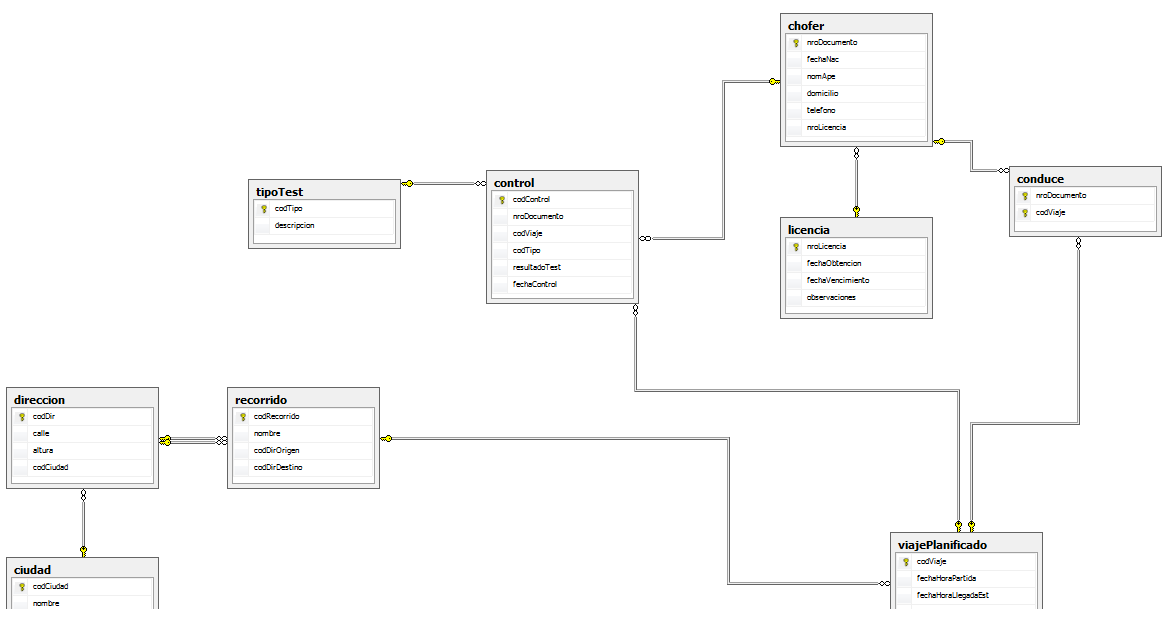
\includegraphics[scale=0.50]{img/DiagramaBaseFisica1.png}}
\end{center}

\begin{center}
\fbox{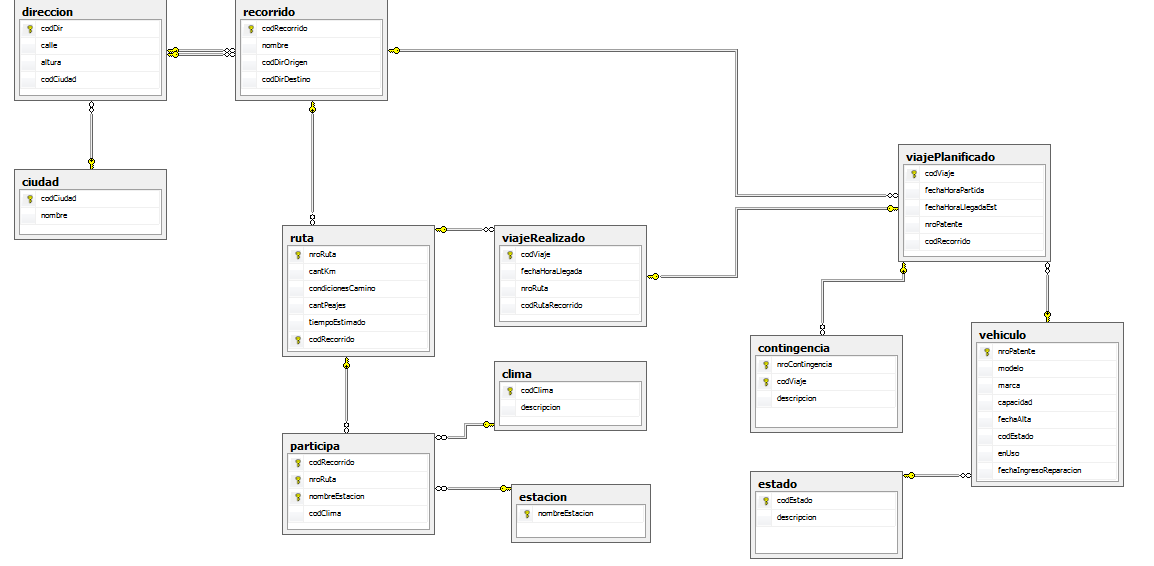
\includegraphics[scale=0.50]{img/DiagramaBaseFisica2.png}}
\end{center}

\subsection{Scripts}
En esta secci�n explicaremos con m�s detalle los scripts mencionados con anterioridad, incluyendo los motivos de su creaci�n en funci�n de las necesidades del presente trabajo pr�ctico.

\subsubsection{Creaci�n de la Base}
En el script \textbf{BD-CreacionBase} solo se hace el `''create database BDtp1Grupo1" para crear una base de datos con el nombre BDtp1Grupo1.

\subsubsection{Creaci�n de Tablas}
Para esto se utiliz� el script \textbf{BD-CreacionTablas}.\\
Al momento de la creacion de la estructura de la base de datos se tomaron las siguientes decisiones:
\\ 

Se crearon las siguientes tablas:
	\begin{itemize}
		\item \textbf{Licencia}: Representa la licencia de conducir de un chofer.
		\item \textbf{Chofer}: Representa un chofer el cual tiene asociada una licencia que debe estar creada antes de crear el chofer. No se puede crear un chofer sin una licencia.
		\item \textbf{ViajePlanificado}: Representa un viaje planificado que pudo o no haber sido realizado dependiendo de si existe un registro relacionado en la tabla viajeRealizado.
		\item \textbf{Conduce}: Relaciona un viaje con N choferes.
		\item \textbf{Control}: Representa el control realizado a un chofer en particular para un determinado viaje y su resultado, es decir, si fue aprobado o no. 
		\item \textbf{TipoTest}: Representa los tipos de test que se le puede hacer a los choferes asignados a un viaje previo a la fecha de partida del mismo. Por ejemplo: alcoholemia, vista, etc.
		\item\textbf{Contingencia}: Representa los posibles eventos que puedan surgir en un viaje que ya lleg� a destino.
		\item \textbf{Direccion}: Representa una calle y una altura, va a representar una punto de partida y de llegada para la tabla recorrido.
\item \textbf{Ciudad}: Representa una ciudad para la cual se definir�n N registros en la tabla direccion.
\item \textbf{Recorrido}: Es una tabla que vincula dos direcciones, una de origen y otra de destino.
\item \textbf{Ruta}: Esta tabla contiene un registro por cada ruta posible para un recorrido.
\item \textbf{Estado}: Refleja los posibles estados de un vehiculo.
\item \textbf{Vehiculo}: Esta tabla representa todos los vehiculos, tanto en uso como en reparaci�n.
\item \textbf{ViajeRealizado}: Tabla relacionada con la tabla ViajePlanificado, contiene los datos propios de un viaje que ya fue realizado.
\item \textbf{Participa}: Relaciona las tablas Clima, Estacion y Ruta. Para cada Ruta y cada Estacion debe haber un registro con el Clima de dicha Ruta en dicha Estacion.
\item \textbf{Estacion}: Representa las 4 estaciones del a�o.
\item \textbf{Clima}: Representa los posibles climas.
\end{itemize}

Se decidi� crear una sola tabla para representar todos los veh�culos (tabla vehiculo), tanto los que est�n en reparaci�n como los que est�n en uso, ya que la �nica diferencia entre ellos es un campo de tipo fecha.
En este caso, como la herencia de vehiculo a vehiculoEnUso y vehiculoEnReparacion es dijunta se utiliza un campo, cuyo nombre es enUso, que admite 2 valores (0 si el vehiculo est� en reparaci�n y 1 si el vehiculo esta en uso).
Luego, a trav�s de un constraint en la tabla, restringimos que si un vehiculo tiene un 0 en el campo enUso entonces debe tener fecha de ingreso a reparacion (campo fechaIngresoReparacion) y esta fecha debe ser posterior a la fecha de alta del vehiculo (fechaAlta). 


\subsubsection{Agregado de restricciones}
Para el agregado de constraints se emple� el script \textbf{BD-AgregadoConstraits}.\\
Se agregaron constraints en las tablas de licencia, en la de vehiculo y la tabla recorrido que restringe el ingreso de datos comparando datos en campos de la misma tabla.\\
Las constraints que se incluyeron en las tablas son las sigueintes:
\begin{itemize}
\item A- alter table licencia add constraint fechaVencimientoMayorAFechaObtencion check (fechaVencimiento > fechaObtencion)\\
	Evita tener licencias con fecha de vencimiento menor a la fecha de obtencion
\item B- alter table vehiculo add constraint verificacionEnUso check ((enUso = 1 and fechaIngresoReparacion is null) or (enUso = 0 and fechaIngresoReparacion is not null and fechaIngresoReparacion >= fechaAlta))\\
	Restringe que si un vehiculo esta en reparacion no tenga dato en la fecha de ingreso a reparacion y lo contrario para uno que esta en uso.
\item C- alter table recorrido add constraint direccionesDistintas check (not (codDirOrigen = codDirDestino))\\
	Restringe que un recorrido tenga igual direccion de origen y destino.
\end{itemize}

\subsubsection{Agregado de triggers}
Esto se hizo mediante el script \textbf{BD-AgregadoTriggers}\\
Se agregaron los siguientes triggers para validar la inserci�n y actualizaci�n de datos en viajePlanificado y la actualizacion de vehiculos. 
Estos triggers cumplen con el requerimiento de \textit{'Implementaci�n de alguna restricci�n adicional que surja del dise�o'}.\\
Hay otras restricciones(ej: que al asociar un chofer a un viaje planificado a trav�s de la tabla Conduce no haya 3 choferes ya asociados a ese viaje) que no fueron implementadas.\\
Con el siguiente script se valida que el viaje que se est� insertando est� asociado a un vehiculo que en uso.

\begin{verbatim}
exec ('CREATE TRIGGER nuevoViaje
ON viajePlanificado
FOR INSERT
AS
/* Chequeamos que enUso del vehiculo asociado al viaje sea distinto a 0, 
para que sea una insercion valida. */
DECLARE @enUso bit
SELECT @enUso = v.enUso
FROM vehiculo v INNER JOIN inserted vp ON v.nroPatente = vp.nroPatente
IF @enUso = 0 
BEGIN
  RAISERROR (''No se puede insertar un viaje planificado asociado a un vehiculo en reparacion.'', 16, 1)
  ROLLBACK TRANSACTION
END')
\end{verbatim}

Con el siguiente script se valida que el viaje que se est� actualizando no haya sido realizado.
\begin{verbatim}
exec ('CREATE TRIGGER actualizarViaje
ON viajePlanificado
FOR update
AS
/* Chequeamos si existe un viaje realizado para el viaje planificado. 
Si es as�, no permitimos la actualizaci�n.*/

if exists (select * from viajeRealizado vr inner join inserted vp on vr.codViaje = vp.codViaje)
BEGIN
   RAISERROR (''No se puede modificar el viaje realizado.'',16,1)
   ROLLBACK TRANSACTION
END')

\end{verbatim}

Con el siguiente script se valida que el vehiculo que se est� modificando, pasando a estar en reparaci�n, no tenga asociado un viaje planificado que todav�a no se haya realizado.
\begin{verbatim}
/*
	Impide poner un auto en reparacion si tiene asociado un viaje planificado que todav�a no se realiz�
*/
exec ('CREATE TRIGGER actualizarVehiculo
ON vehiculo
FOR update
AS
/* Chequeamos si el vehiculo tiene un viaje planificado asociado y no un viaje realizado. 
Si es as�, no permitimos la actualizacion.*/
if	exists (select * from inserted v where enUso=0 and
		exists(	select * from viajePlanificado vp 
				where vp.nroPatente = v.nroPatente and 
				not
					exists(select * from viajeRealizado vr where vr.codViaje=vp.codViaje)
				)
	)
BEGIN
   RAISERROR (''No se puede configurar un vehiculo como en reparacion que 
   est� asignado a un viaje planificado.'', 16, 1)
   ROLLBACK TRANSACTION
END')
\end{verbatim}

\subsubsection{Creaci�n de Vistas}
Mediante el script \textbf{BD-CreacionVistas}.\\
Para resolver algunos de los requerimientos del enunciado se crearon vistas a tablas de la base de datos:

\begin{itemize}
\item \textit {\textbf{`'Los recorridos para los cuales se usaron todas las rutas posibles registradas para ese recorrido, para viajes realizados el a�o pasado y recorridos asociados a m�s de una ruta"}}.\\
\\
Se implement� la vista \textbf{recorridosConTodasRutasUsadasAnioAnterior} que cumple con el requerimiento de listar `'Los recorridos para los cuales se usaron todas las rutas posibles registradas para ese recorrido, para viajes realizados el a�o pasado y recorridos asociados a m�s de una ruta".
\\
Esta vista utiliza las siguientes dos vistas auxiliares: 
\begin{itemize}
\item \textbf{cantRutasXRecorrido}, que cuenta la cantidad de rutas de un recorrido y
\item \textbf{cantRutasRecorridasAnioAnterior}, que cuenta las rutas distintas que se utilizaron para realizar cada recorrido.
\end{itemize}
Debajo se adjuntan las implementaciones de cada una de las vistas:
\\
\begin{verbatim}
exec ('create view recorridosConTodasRutasUsadasAnioAnterior as 
(select  crraa.codRutaRecorrido as codRecorrido , crxr.nombre as recorrido  
from cantRutasXRecorrido crxr join cantRutasRecorridasAnioAnterior crraa
on crxr.recorridoRutas = crraa.codRutaRecorrido 
where cantRutasRec = rutasRecorridasAnioAnt)')

/*
	Se crea la vista cantRutasXRecorrido devuelve el c�digo de recorrido y 
	la cantidad de rutas distintas que se utilizaron
	en los viajes del a�o anterior.
*/
exec ('create view cantRutasXRecorrido as 
(select count(*) as cantRutasRec,rec.codRecorrido as RecorridoRutas,rec.nombre 
from recorrido rec join ruta on rec.codRecorrido = ruta.codRecorrido 
group by rec.codRecorrido,rec.nombre having count(*) > 1)')


/*
	Se crea la vista cantRutasRecorridasAnioAnterior devuelve el nombre del recorrido, el c�digo 
	y la cantidad de rutas asociadas
*/

exec ('create view cantRutasRecorridasAnioAnterior as 
(select count(*) as rutasRecorridasAnioAnt , codRutaRecorrido 
from (select distinct r.nroRuta , vr.codRutaRecorrido   from ruta r, 
viajeRealizado vr 
where (year(GETDATE())-1)= year(fechaHoraLlegada) and 
r.codRecorrido = vr.codRutaRecorrido and r.nroRuta = vr.nroRuta)
as rutasTransitadasXRec  group by codRUtaRecorrido)')
\end{verbatim}

\item \textit{\textbf{`El promedio de viajes realizados por veh�culo por a�o y el estado en que �ste se encuentra"}}.\\
\\
Adem�s, se implement� la vista \textbf{promedioEstadoXVehiculo} para cumplir con el requerimiento de listar `'El promedio de viajes realizados por veh�culo por a�o y el estado en que �ste se encuentra".\\
Esta vista utiliza la vista auxiliar \textbf{cantViajesXVehiculoXAnio} que devuelve la cantidad de viajes de cada vehiculo por cada a�o de actividad. \\
Debajo se adjuntan las implementaciones de cada una de las vistas:
\\
\begin{verbatim}
exec ('create view promedioEstadoXVehiculo as (select auxQuery.nroPatente, auxQuery.promedioXAnio,
 estado.descripcion
from (
-- Este subquery devuelve el promedio de viajes x anio para cada vehiculo
	select auxView.nroPatente, AVG(cast(auxView.viajesXAnio as money))as promedioXAnio
	from cantViajesXVehiculoXAnio as auxView
	group by auxView.nroPatente
) as auxQuery
-- Agrego la informaci�n del estado actual del vehiculo
join vehiculo on auxQuery.nroPatente = vehiculo.nroPatente
join estado on vehiculo.codEstado = estado.codEstado)')

/*
	Se crea la vista cantViajesXVehiculoXAnio que devuelve para cada vehiculo, 
	la cantidad de viajes ya realizados por cada a�o
*/
exec ('
CREATE view cantViajesXVehiculoXAnio as 
(select vehiculo.nroPatente, DATEPART(year, vP.fechaHoraPartida) as anio,
 count(vP.codViaje) as viajesXAnio
	from viajeRealizado vR join viajePlanificado vP on vR.codViaje = vP.codViaje
	join vehiculo on vP.nroPatente = vehiculo.nroPatente
	group by vehiculo.nroPatente, DATEPART(year, vP.fechaHoraPartida))')

\end{verbatim}

\item \textit{\textbf{Los choferes que han utilizado todos los veh�culos de menos de dos a�os de antig�edad, en viajes del �ltimo semestre}}.\\
\\
Por ultimo, se implement� la vista \textbf{chofer6MVehiculo2A} que devuelve `'Los choferes que han utilizado todos los veh�culos de menos de dos a�os de antig�edad, en viajes del �ltimo semestre."
Esta vista utiliza las siguientes vistas auxiliares: 
\begin{itemize}
\item \textbf{patenteXviajesRealizados}: muestra los viajes realizados por cada vehiculo,
\item \textbf{viajesUltimos6Meses}: devuelve todos los vehiculos usados por cada chofer en los ultimos 6 meses, 
\item \textbf{antiguedadXVehiculo}: muestra el numero de patente y la antiguedad de cada vehiculo y
\item \textbf{viajesChoferesUltimos6Meses}: filtra los viajes realizados por los choferes qued�ndose con los que fueron realizados en los �ltimos 6 meses.   
\end{itemize}

Debajo se adjuntan las implementaciones de cada una de ellas:

\begin{verbatim}
exec ('CREATE view chofer6MVehiculo2A as
select v.nroDocumento, v.nomApe from viajesChoferesUltimos6Meses v where exists
(select 1 from antiguedadXVehiculo where antiguedadXVehiculo.antiguedad<2 having
 count(*)=v.cantVehiculos)')

/*
	Viajes planificados y realizados y patente del vehiculo que realiz� el viaje
*/

exec ('create view patenteXviajesRealizados as (select vr.codViaje,vr.fechaHoraLlegada,
 vp.nroPatente as patente 
from viajePlanificado vp inner join viajeRealizado vr on vp.codViaje = vr.codviaje)')

/*
	Todos los vehiculos usados por cada chofer en los ultimos 6 meses.
*/

exec ('create view viajesUltimos6Meses as
select * from patenteXviajesRealizados where dateadd(month, 6, fechaHoraLlegada) > getdate() ')

/*
	Creamos una vista que devuelve el numero de patente y la antiguedad de los vehiculos
*/
exec ('create view antiguedadXVehiculo as select nroPatente , (DATEDIFF(yy, fechaAlta, GETDATE()) -
CASE WHEN MONTH(fechaAlta) > MONTH(GETDATE()) OR (MONTH(fechaAlta) =
MONTH(GETDATE()) AND DAY(fechaAlta) > DAY(GETDATE()))
THEN 1 ELSE 0 END) as antiguedad from vehiculo')

/*
	Lista los choferes y cantidad de vehiculos distintos que manej� cada chofer en los ultimos 6 meses.
*/

exec ('create view viajesChoferesUltimos6Meses as
select nroDocumento, nomApe, count(*) as cantVehiculos from
	(	select distinct c.nroDocumento, c.nomApe, vp.nroPatente
		from chofer c join conduce co on co.nroDocumento=c.nroDocumento join viajePlanificado vp on
		 vp.codViaje=co.codViaje 
		where exists (select 1 from viajesUltimos6Meses v6m where v6m.codViaje=vp.codViaje)
	) as auxQuery
group by nroDocumento, nomApe')
\end{verbatim}
\end{itemize}

\subsubsection{Inserci�n de datos}
Mediante el script \textbf{BD-InsercionDatos}.\\
Este script inserta datos para los cuales se pueden probar cada uno de los requerimientos del enunciado y las restricciones insertadas mediante triggers y constraints en las distintas tablas.
Como tambi�n, se pueden obtener resultados para las vistas `'recorridosConTodasRutasUsadasAnioAnterior", `'promedioEstadoXVehiculo" y `'chofer6MVehiculo2A".


\subsection{Aclaraciones adicionales}
\begin{itemize}
	\item En la tabla \textbf{control} el campo \textit{resultadoTest} es de tipo bit ya que los test pueden estar aprobados o desaprobador. Es decir toma los valores $0$ y $1$, donde $1$ significa aprobado y $0$ significa desaprobado.
	\item Los vehiculos pueden estar \textbf{en uso} o \textbf{en reparaci�n}. En la tabla \textbf{vehiculo} se tiene un campo llamado \textit{EnUso}. Este campo es de tipo bit ya que toma solo dos valores: $1$ significa en uso y $0$ significa en reparaci�n.
	\item En todos los campos de tipo char, estos se tomaron de longitud 30.   
\end{itemize}


\end{document}




